\subsection{清明节}

清明节又叫踏青节,在仲春与暮春之交,一般在公历4月5日前后,春分后第15日。清明节是中国的传统节日之一,国家规定假期为每年的4月5日至4月7日。清明节不单单只有中国人过节,在其他亚洲国家,如越南、韩国等也会过清明节。

清明节历史悠久,既是节气又是节日,节日习俗的形成与此时的节气特点密切相关。节气为节日的产生提供了前题条件。清明为中国二十四节气之一,时间约在每年的冬至后第108天,也就是阳历4月5日前后。二十四节气是上古时期古人依据地球在黄道上的位置变化而制定的气候规律,比较客观地反映了一年四季气温、物候、降雨等方面的变化,对人们依时安排农事生产活动有不可或缺的指导意义。清明节后气温变暖,雨水增多,大地呈现春和景明之象。这一时节万物“吐故纳新”,无论是大自然中的植被,还是与自然共处的人体,都在此时换去冬天的污浊,迎来春天的气息,实现由阴到阳的转化。所以清明对于古代农事生产而言是一个重要的节气。清明作为节日,与纯粹的节气又有所不同,节气是我国物候变化、时令顺序的标志,而节日则包含着一定的风俗活动和某种纪念意义。

清明节扫墓祭祖礼俗的源流与信仰、祭祀、历法以及划分出的节气等人文与自然文化内容有关。清明节气在时间和气象物候特点上为清明节俗的形成提供了重要条件,该节气被看作清明节的源流之一。清明时节,大地呈春,阴阳转化,吐故纳新,生气始盛,万物皆洁齐,正是春祭好时段。同时郊外踏青也是古人们的节气主题。古时代农业是传统社会的主业,为了农事的丰收,除了祈求自然风调雨顺外,还得请祖先保佑,并且国人自古就有礼敬祖先、慎终追远的礼俗观念。因此在清明时节逐渐形成春祭的传统。经历史发展演变,清明节吸收融合了寒食节与上巳节的习俗,具有极为丰富的文化内涵。
\begin{figure}[htb]
    \centering
    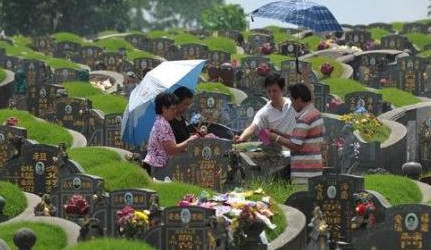
\includegraphics[width=0.6\linewidth]{shaomu}
    \caption{扫墓}
\end{figure}


清明节是中国的祭祀节日。“祭祀”即是悼念先人之节,是和祭祀天神、地神的节日相对而言的。清明祭祀的参与者是全体国民,上至君王大臣,下至平头百姓,都要在这一节日祭拜先人。清明扫墓,谓之对祖先的“思时之敬”。其习俗由来已久。清明节的祭祖习俗,据传始于古代帝王将相郊外踏青时举行“墓祭”之礼,后来民间亦相仿效,于此日扫墓祭祖。唐人沿袭前代祭墓风俗,并扩大到整个社会。从《礼经》的记载看,古代北方中原并没有清明上墓祭扫的例规,但唐时已成风气。从唐朝开始,朝廷就给官员放假以便于归乡扫墓。据宋《梦粱录》记载:每到清明节,“官员士庶俱出郊省墓,以尽思时之敬。”参加扫墓者也不限男女和人数,往往倾家出动。这样清明前后的扫墓活动常成为社会全体亲身参与的事,数日内郊野间人群往来不绝,规模极盛。作为祭祀,清明之祭主要祭祀祖先,表达祭祀者的孝道和对先人的思念之情。清明节属于祭祀节而通常不被冠以鬼节之名,就在于它重在表达孝思亲情。清明祭祀在清明前后,各地有所差异。清明祭祀按祭祀场所的不同可分为墓祭、祠堂祭。以墓祭最为普遍,清明祭祀的特色就是墓祭,清明祭祀被称为扫墓,主要是由于采取墓祭方式。另一种形式是祠堂祭,又称庙祭,是一个宗族的人聚集在祠堂共祭祖先,祭完后要开会聚餐等,这种祭祀是团聚族人的一种方式。还有一种情况是家在外地工作的人不能赶回家乡扫墓,就在山上或高处面对家乡的方向遥祭。

\begin{figure}
    \centering
    \includegraphics[width=0.8\linewidth]{qingmingshanghetu}
    \caption{北宋时期名画——清明上河图}
\end{figure}
\subsubsection{传统习俗}
\begin{enumerate}
\item 
清明节扫墓祭祖的节俗传统自古持续不断,就是到了当今的社会,人们在清明节前后仍有上坟扫墓祭祖的习俗:铲除杂草,放上供品,于墓前上香祷祝、燃纸钱金锭等,又或简单地献上一束鲜花,以寄托对祖先的追念。
\item 
清明踏青也叫春游,古代叫探春、寻春;其含义,就是脚踏青草,在郊野游玩,观赏春色。清明之时,正值春回大地,人们乃因利趁便,扫墓祭祖之余亦一家老少在山乡野间游乐一番。踏青与祭祖是清明节最早的习俗,随着历史的推移,不少地方家族观念和祭祖观念正日渐淡薄,这类活动现已大多式微。古时扫墓祭祖的传统习俗至今在岭南一带仍盛行,自古传承至今不辍,每逢清明时节,人们无论身处何方,都会回乡参加祭祖活动。清明节不仅是人们祭祀祖先的节日,也是中华民族认祖归宗的纽带。清明节俗丰富,但归纳起来是两大节令传统:一是礼敬祖先,慎终追远;二是踏青郊游、亲近自然。
\item 
清明前后,春阳照临,春雨飞洒,种植树苗成活率高,成长快。因此,就有清明植树的习惯,有人还把清明节叫作“植树节”。植树风俗一直流传至今。清明节植树的习俗,据说发端于清明戴柳插柳的风俗。关于清明戴柳插柳,有三种传说。第一种传说,据说是为了纪念教民稼穑耕作的祖师—神农氏,后来由此发展出祈求长寿的意蕴。第二种传说与介子推有关,据说晋文公率众臣登山祭奠介子推时,发现介子推死前曾经靠过的老柳树死而复活,便赐老柳树为“清明柳”。第三种传说是唐太宗给大臣柳圈,以示赐福驱疫。    
\end{enumerate}

\subsubsection{节令食品的南北差异}
北方一些地方还保留着清明节吃冷食的习惯。在山东,即墨吃鸡蛋和冷饽饽,莱阳、招远、长岛吃鸡蛋和冷高粱米饭,据说不这样的话就会遭冰雹。泰安吃冷煎饼卷生苦菜,据说吃了眼睛明亮。晋中一带还保留着清明前一日禁火的习惯。很多地方在完成祭祀仪式后,将祭祀食品分吃。晋南人过清明时,习惯用白面蒸大馍,中间夹有核桃、枣儿、豆子,外面盘成龙形,龙身中间扎一个鸡蛋,名为“子福”。要蒸一个很大的总“子福”,象征全家团圆幸福。上坟时,将总“子福”献给祖灵,扫墓完毕后全家分食之。上海旧俗,用柳条将祭祀用过的蒸糕饼团贯穿起来,晾干后存放着,到立夏那天,将之油煎,给小孩吃,据说吃了以后不得疰夏病。部分地区清明节时有吃青团的风俗,青团又称清明饼、棉菜馍糍、茨壳粿、清明粑、艾叶粑粑、艾糍、清明果、菠菠粿、清明粿、艾叶糍粑、艾粄、艾草糕、清明团子、暖菇包、艾草青团、清明团子等等。将雀麦草汁和糯米一起舂合,使青汁和米粉相互融合,然后包上豆沙、枣泥等馅料,用芦叶垫底,放到蒸笼内。蒸熟出笼的青团色泽鲜绿,香气扑鼻,是本地清明节最有特色的节令食品。上海也有的人家清明节爱吃桃花粥,在扫墓和家宴上爱用刀鱼。

\begin{figure}
\centering
\includegraphics[width=0.45\linewidth]{qingtuan} 
\includegraphics[width=0.45\linewidth]{qingtuan2}   
\caption{清明的青团}
\end{figure}

\paragraph{节气俗语:}
\begin{itemize}
\item
雨打清明前,春雨定频繁(鲁)
\item 
阴雨下了清明节,断断续续三个月(桂)
\item
清明难得晴,谷雨难得阴(鲁)
\item   
清明不怕晴,谷雨不怕雨(黑)
\item 
雨打清明前,洼地好种田(黑)
\item 
清明雨星星,一棵高粱打一升(黑)
\item 
清明宜晴,谷雨宜雨(赣)
\item 
清明断雪,谷雨断霜(华东、华中、华南、四川及云贵高原)
\item 
清明断雪不断雪,谷雨断霜不断霜(冀、晋)
\item 
清明无雨旱黄梅,清明有雨水黄梅(苏、鄂) 
\end{itemize}